% !TEX root = ../Thesis.tex
\chapter{Introduction}

Page-based virtual memory transparently allocates different parts of the physical memory to each process in units of fixed-sized pages, which are 4KB in nearly all modern systems. The translations between virtual and physical addresses are stored in a hierarchy of page tables (4 levels in modern AMD64 systems). Each page table is a list of page table entries (PTEs) that contain a pointer to the next level or the final physical address. Some architectures, including AMD64, support creating superpages (sometimes known as large pages or huge pages) by setting a flag in the page table entry that stops the page table walk before the final level. The resulting superpages are thus 2MB or 1GB in size on AMD64.

The Translation Lookaside Buffer (TLB) caches virtual-to-physical translations so that the memory-management unit (MMU) does not need to walk the page tables for every memory access. The TLB is critical to performance and TLB misses add significant overhead to execution time in many workloads \cite{Barr}. Superpages offer a reduction in TLB misses by allowing larger regions of memory to be represented with one TLB entry. The TLB has separate groups of entries for 2MB, 1GB, and the regular 4KB pages. In addition to reducing TLB misses, superpages make the cost of a TLB miss slightly smaller because the page table walk only has three steps instead of four.

While superpages can increase TLB reach and thus reduce misses, they are less flexible than 4KB pages (small pages) because they map a larger contiguous region of memory. PTEs include flags that mark various properties of the page, such as whether or not it has a mapping to physical memory, whether it is writeable or read-only, and whether it is accessible to the user or only the kernel. Since these flags apply to the entire region mapped by a PTE, small pages allow much finer-grained management than superpages.

The Linux kernel has a system called Transparent Hugepages (THP) which automatically creates 2MB superpages whenever large blocks of memory are allocated or previously-allocated blocks of memory are found to be aligned to 2MB \cite{THP}. This enables any program to gain the advantages of superpages without being written with them in mind. To maintain transparency to userspace, THP are automatically split whenever an operation is done that would change the flags of one of the pages it contains.

The goal of this paper is to demonstrate a method to gain most of the advantages of superpages (fewer TLB misses and faster page table walks) while avoiding most of the disadvantages (less flexibility).

\section{Copy-On-Write}

The main operation this paper investigates is copy-on-write (COW), where two processes map a page of their virtual address space to the same physical frame until one process tries to write to the page. The page is marked read-only so that this write causes a page fault, allowing the kernel to handle it. When that happens, the page is copied, the writing process changes its mapping to the new page, and only the new page receives the write. This allows processes to share as much memory as possible, reducing memory usage and increasing performance. With superpages, much of this benefit is lost because even a small write forces the entire large region to be copied. Alternatively, a transparent hugepage could be split when a COW occurs to allow only 4KB to be copied at a time, but this gives up the TLB miss savings. Transparent hugepages are not currently split by default for COW.

COW is most commonly used whenever a program forks to create a new process. The child process shares its parent's address space until writes trigger the COW mechanism for each page. This makes the fork operation much faster than it would be if the whole address space was copied, and it reduces memory usage by never duplicating sections of memory that do not change.

Another possible application of COW is in memory checkpointing. It may be useful to take periodic snapshots of the memory of a system, to allow error recovery, backups, or speculative changes. A simple way to accomplish this is to write-protect the entire address space at the start of a checkpoint and use COW to allow the program to continue normal execution while another process writes out the memory to a different location \cite{Sun}.

Copy-on-write is one of the most common operations where the loss of flexibility caused by superpages significantly limits their usefulness.

\section{Prior Work}

Other groups have proposed ways to gain most of the benefits of superpages without the downsides. The GLUE \cite{Pham} and SpecTLB \cite{Barr} systems both use speculative TLB entries to map 2MB regions of virtual addresses that are mostly aligned. GLUE is software-transparent, which means that the TLB automatically creates speculative entries and the operating system does not need to be changed to support it. SpecTLB, on the other hand, requires minor operating system changes to explicitly mark speculative superpages. Since both of these systems are speculative in nature, there are some major downsides. A speculation failure will incur a significant overhead to roll back everything the processor did with the incorrect translation, and the infrastructure required to do so complicates the entire memory management system. However, they do show significant reductions in TLB misses as a result of improved superpage utilization.

\section{Superpage Overlays}

Our proposed solution to the downsides of superpages is to use a system called ``overlays'' to allow more flexible management of superpages and achieve the best of both worlds. In addition to the existing mapping from a virtual superpage to contiguous physical memory, each small page within the superpage can optionally map to an overlay, which overrides the virtual-to-physical mapping for that page (see figure \ref{fig:basic}). The set of pages within a superpage that map to overlays is defined by the overlay bit vector (OBitVector), and they are mapped via a second page table called the overlay mapping table (OMT). With this system, copy-on-write can be replaced with overlay-on-write. Instead of copying the entire superpage, an overlay is created for one small page in the address space of the writing process. Thus, only 4KB needs to be copied and the rest of the superpage still exists for both processes, providing the usual memory utilization and TLB reach improvements.

The superpage overlay system presented here is based on page overlays from another recent work \cite{Seshadri}. That framework used overlays the size of a cache line for very fine-grained management of regular pages. Superpage overlays are simpler in that they can simply extend the existing page table system and thus require less significant changes to the MMU.

Compared to the prior work, superpage overlays have the substantial advantage of not using speculative translations. Any TLB hit is guaranteed to be correct. This simplifies the memory management hardware and eliminates the overhead of a failed speculation. Another difference is that superpage overlays require significant changes to the operating system. The OS must maintain the OMT as well as the page tables, and it must explicitly create the overlays.

This project makes three main contributions. First, we describe the superpage overlay framework and show how it would be implemented. Second, we describe the trap-driven simulation infrastructure that can be used to test the effectiveness of superpage overlays without using the modified hardware that the framework requires. Third, we show the benefits of superpage overlays for some example applications.

\begin{figure}
    \centering
    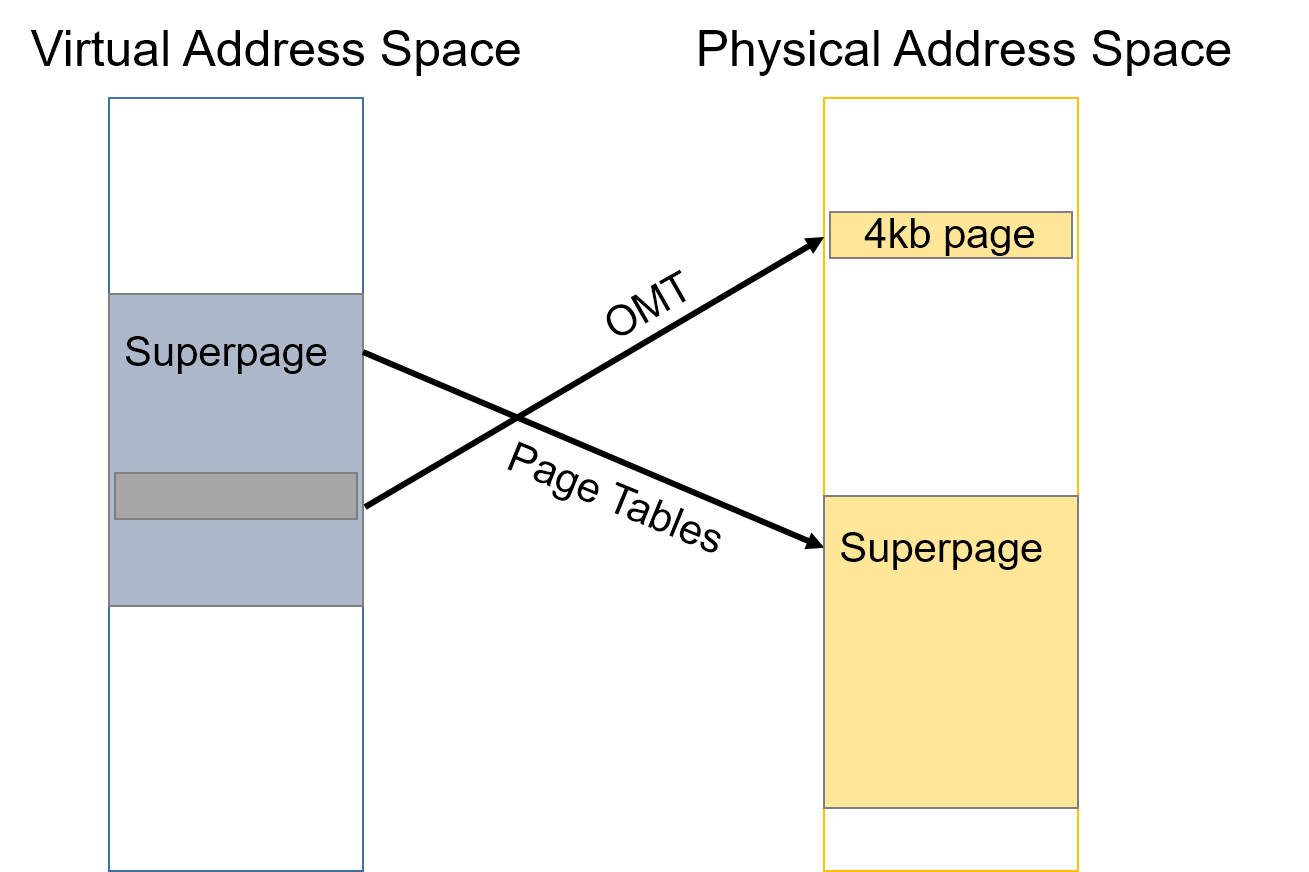
\includegraphics[width=2.5in]{Figures/Picture1}
    \caption{A basic diagram of the virtual-to-physical mappings for a superpage with overlay}
    \label{fig:basic}
\end{figure}
